\begin{frame}
\frametitle{The need of Quantum Field Theory}
In spite of the heroic efforts of Dirac and others, RQM is not enough to describe elementary particles. The Dirc equation describes a single electron. Positrons need to be introduced by a sort of magical incantation (the negative sea state). In short, RQM cannot predict creation and annihilation of particles. 

Quantum Electrodynamics (QED) was eventually developed as the first Quantum Field Theory (QFT), capable of describing such creation and annihilation of particles. In QED, it is not only the photons that are quanta of a field but also the charged particles, like the electrons and positrons. The fields are operators that create and annihilate their quanta. \alert{Thus $\psi(x)$~is no longer interpreted as a waveform that describes probability but as an operator that creates a particle in point $x$~and destroys an antiparticle in $x$ ($\bar{\psi}(x)$~will create an antiparticle in point $x$~and destroy antiparticle in $x$)}.

%The Lagrangian of the free Dirac field $\psi$~is given by:
%
%\begin{empheq}[box=\fbox]{align}
%  L = \bar{\psi}(i\gamma^\mu \partial_\mu -m)\psi  \nonumber
%\end{empheq}
%
%where $\bar{\psi} = \psi^\dagger \gamma^0$. Varying the Lagrangian yields back the Dirac equation.

%The $\gamma$~matrices found by Dirac were complex. This means that the spinor field $\psi$~must also be complex. This makes sense from the point of view of field theory as a complex field would create particles and annihilate anti-particles while its complex conjugate would create anti-particles and annihilate particles. However, as we shall see, Majorana found an alternative. 

\end{frame}

\begin{frame}
\frametitle{Feynman Diagrams}
\begin{columns}
\column{0.4\textwidth}
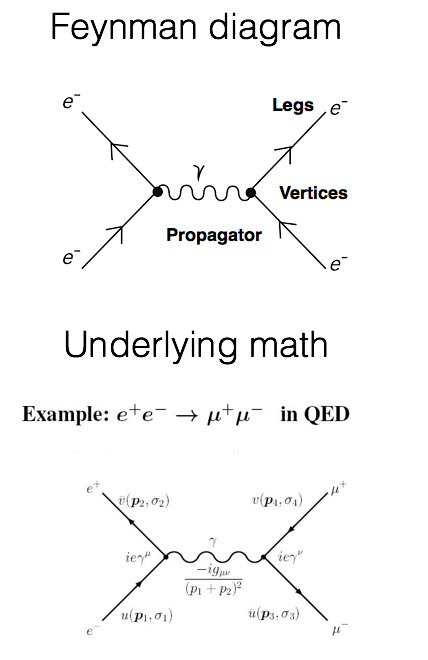
\includegraphics[scale=0.3]{FeynmanD2.png}
 
\column{0.5\textwidth}
Feynman diagrams: ``pictures'' whose lines are world-lines of the particles in the space-time. They are representations of mathematical expressions of scattering or decay amplitudes. We cannot do the math here, but the diagrams suggest nicely the underlying physics. 

\end{columns}
\end{frame}
\begin{frame}
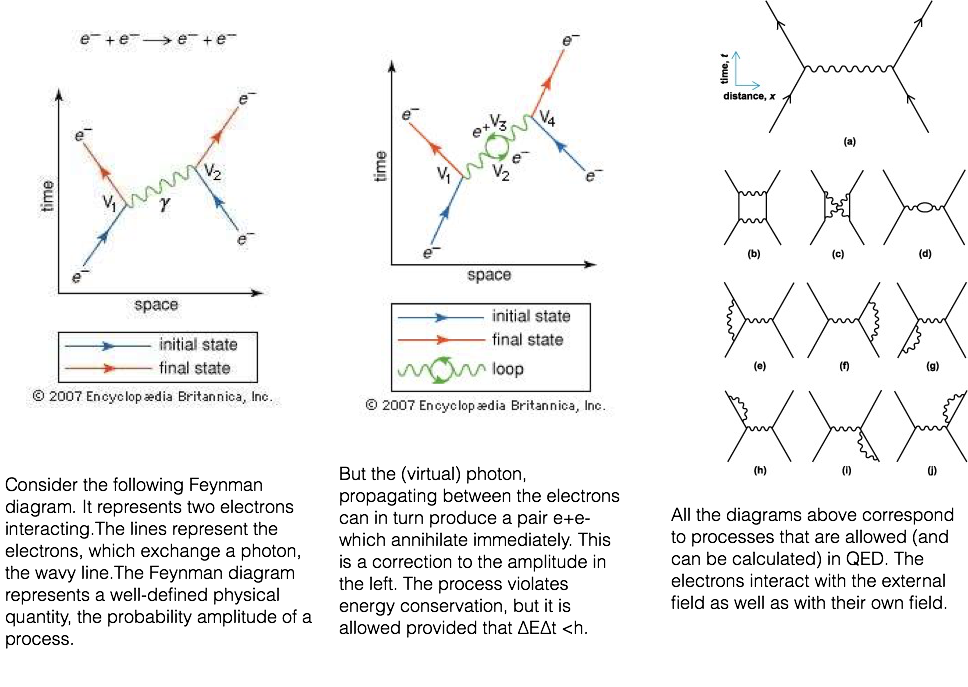
\includegraphics[scale=0.3]{FeynmanD3.png}

\end{frame}